\documentclass[
	aspectratio=169, % default is 43
	8pt, % font size, default is 11pt
	%handout, % handout mode without animations, comment out to add animations
]{beamer}
\def\university{}

\documentclass[
	aspectratio=169, % default is 43
	8pt, % font size, default is 11pt
	handout, % handout mode without animations, comment out to add animations
]{beamer}

\usepackage{../template/beamerthemeuulm} % use the inofficial uulm beamer theme
\setfaculty{infIngPsy} % set the color scheme for your faculty here [med/infIngPsy/math/nat]

% requires symbolic links
% git clone git@github.com:SoftVarE-Group/SlideTemplate.git C:\Users\...\SlideTemplate
% mklink /J template C:\Users\...\SlideTemplate
% git clone git@spgit.informatik.uni-ulm.de:thuem/slides.git C:\Users\...\ThomasSlides
% mklink /J thomasslides C:\Users\...\ThomasSlides
\graphicspath{{../template/pics/logos}{../template/pics/nature}{../template/pics/uulm}{../thomasslides/}{../pics/people/}{../pics/xkcd/}}

%\usepackage[ngerman]{babel} % use this line for slides in German
%\recordingtrue % special recording mode for use with a greenscreen, gives you space to show yourself in a layer in front of the slides, has no effect in the handout mode

\title{Software Product Lines} % short title is used for the slide footer but optional

% LINKED LITERATURE

\newcommand{\ludewiglichter}{\href{https://learning.oreilly.com/library/view/-/9781457184932/?ar}{Ludewig and Lichter}}
\newcommand{\seeconomics}{\href{https://rds-ulm.ibs-bw.de/link?kid=027381854}{SE Economics}}
\newcommand{\sommervillelink}[1]{\href{https://ulm.ibs-bw.de/aDISWeb/app?service=direct/0/Home/$DirectLink\&sp=SOPAC00\&sp=SAKSWB-IdNr1615420983}{#1}}
\newcommand{\sommerville}{\sommervillelink{Sommerville}}
\newcommand{\thehumbleprogrammer}{\href{https://dl.acm.org/doi/10.1145/1283920.1283927}{The Humble Programmer}}
\newcommand{\thepragmaticprogrammer}{\href{https://learning.oreilly.com/library/view/the-pragmatic-programmer/9780135956977/}{The Pragmatic Programmer}}

% TYPICAL COMMANDS FOR LECTURES

\renewcommand{\emph}[1]{{\color{blue}\textbf{#1}}}

\newcommand{\deutsch}[1]{{\color{blue}(#1)}}
\newcommand{\deutschertitel}[1]{{\tiny\deutsch{#1}}}

\newcommand{\mycite}[1]{``#1''}
\newcommand{\mytitlesource}[1]{{\tiny\normalfont\mbox{[#1]}}}
\newcommand{\mysource}[1]{\ifthenelse{\equal{#1}{}}{}{\phantom{.}~\hfill~\mytitlesource{#1}}}

\newcommand{\todo}[1]{{\color{red}\textbf{[#1]}}}
\newcommand{\fodo}[1]{\todo{\footnote{\todo{#1}}}}
\newcommand{\todots}{\todo{\ldots}}

% IMPORTED PACKAGES

%\usepackage{adjustbox} % used for partofpage
%\usepackage{tcolorbox} % used for mydefinition, mynote, myexample
\usepackage{multicol} % used temporarily for the lecture overview
\usepackage{mathtools} % required for absolute value in modeling lecture

% COMMANDS TO LAYOUT AND ANNIMATE SLIDES

\newcommand{\lessonslearned}[3]{
	\subsection{Summary}
	\begin{frame}{\insertsection -- \insertsubsection}
		\leftorright{
			\mydefinition{Lessons Learned}{
				\begin{itemize}
					#1
				\end{itemize}
			}
			\mynote{Further Reading}{
				\small % references take space, can be a little smaller
				\begin{itemize}
					#2
				\end{itemize}
			}
		}{
			\myexample{Practice}{
				#3
			}
		}
	\end{frame}
}

% TODO temporary hack to layout the slide overview in two colums
\renewcommand{\lectureoverview}{
%	\section*{Overview}
%	\subsection*{Overview}
	\begin{frame}{\insertsubtitle}
		\begin{multicols}{2}
			\tableofcontents
		\end{multicols}
	\end{frame}
}

\renewcommandx{\maketitle}[2][1=apr21-o25a,2=150]{
    {
	\usebackgroundtemplate{} % TODO temporary hack to enable missing pictures at title slide
	%\ifx {#1} \empty \else {\usebackgroundtemplate{\includegraphics[trim=0 0 0 #2,clip,width=\paperwidth]{#1}}} \fi     
	%\usebackgroundtemplate{\includegraphics[trim=0 0 0 #2,clip,width=\paperwidth]{#1}}
    \begin{frame}[plain]
        \vskip0pt plus 1filll
        \begin{beamercolorbox}[wd=\paperwidth,ht=4.5ex,dp=2ex,right]{titlebox}
            \LARGE\textbf{\inserttitle}\hspace*{20pt}
        \end{beamercolorbox}%
        \nointerlineskip%
        \begin{beamercolorbox}[wd=\paperwidth,ht=2.25ex,dp=1ex,right]{subtitlebox}
            \small 
            \ifx \insertsubtitle \empty \else \insertsubtitle\ $\vert$ \fi
            \insertauthor\
            \ifx \insertdate \empty \else $\vert$ \insertdate \fi
            \hspace*{20pt}
        \end{beamercolorbox}%
        \nointerlineskip%
        \begin{beamercolorbox}[wd=\paperwidth,ht=4.5ex,dp=2ex,left]{logobox}
            \centering
            \vspace{-1ex}
            \hspace{10pt}
            \includegraphics[height=4.5ex]{sp} % SPECIFY INSTITUTE LOGO HERE
            \hfill
            \includegraphics[height=4.5ex]{uulm}
            \hspace{10pt}
        \end{beamercolorbox}%
    \end{frame}
    }  
}

%
%\newcommand{\onlyleft}[1]{
%	\halfpage{#1}
%}
%
%\newcommand{\onlyright}[1]{
%	~\hfill
%	\halfpage{#1}
%}
%
%\newcommand{\leftorright}[2]{
%	\uncover<1>{\halfpage{#1}}
%	\hfill
%	\uncover<3->{\halfpage{#2}}
%}
%
%\newcommand{\rightorleft}[2]{
%	\uncover<3->{\halfpage{#1}}
%	\hfill
%	\uncover<1>{\halfpage{#2}}
%}
%
%\newcommand{\leftthenright}[2]{
%	\halfpage{#1}
%	\hfill\pause
%	\halfpage{#2}
%}
%
%\newcommand{\leftandright}[2]{
%	\halfpage{#1}
%	\hfill
%	\halfpage{#2}
%}
%
%\newcommand{\leftmiddleandright}[3]{
%	\thirdpage{#1}
%	\hfill
%	\thirdpage{#2}
%	\hfill
%	\thirdpage{#3}
%}
%
%\newcommand{\leftmiddleorright}[3]{
%	\uncover<1>{\thirdpage{#1}}
%	\hfill
%	\uncover<3>{\thirdpage{#2}}
%	\hfill
%	\uncover<5->{\thirdpage{#3}}
%}
%
%\newcommand{\halfpage}[1]{\partofpage{48}{#1}}
%
%\newcommand{\thirdpage}[1]{\partofpage{31}{#1}}
%
%\newcommand{\partofpage}[2]{
%	\adjustbox{valign=t}{\begin{minipage}{0.#1\textwidth}
%			\begin{flushleft}
%				#2
%			\end{flushleft}
%	\end{minipage}}
%}
%
%\newcommand{\mydefinition}[2]{
%	\begin{tcolorbox}[title=#1,colback=orange!10,colframe=orange!30,coltitle=black,fonttitle=\bfseries,left=1mm,right=1mm,top=1mm,bottom=1mm]
%		\begin{flushleft}
%			#2
%		\end{flushleft}
%	\end{tcolorbox}
%}
%
%\newcommand{\mydefinitiontight}[2]{
%	\begin{tcolorbox}[title=#1,colback=white,colframe=orange!30,coltitle=black,fonttitle=\bfseries,left=0mm,right=0mm,top=0mm,bottom=0mm]
%		\begin{flushleft}
%			#2
%		\end{flushleft}
%	\end{tcolorbox}
%}
%
%\newcommand{\mynote}[2]{
%	\begin{tcolorbox}[title=#1,colback=red!10,colframe=red!30,coltitle=black,fonttitle=\bfseries,left=1mm,right=1mm,top=1mm,bottom=1mm]
%		\begin{flushleft}
%			#2
%		\end{flushleft}
%	\end{tcolorbox}
%}
%
%\newcommand{\myexample}[2]{
%	\begin{tcolorbox}[title=#1,colback=blue!10,colframe=blue!30,coltitle=black,fonttitle=\bfseries,left=1mm,right=1mm,top=1mm,bottom=1mm]
%		\begin{flushleft}
%			#2
%		\end{flushleft}
%	\end{tcolorbox}
%}
%
%\newcommand{\myexampletight}[2]{
%	\begin{tcolorbox}[title=#1,colback=white,colframe=blue!30,coltitle=black,fonttitle=\bfseries,left=0mm,right=0mm,top=0mm,bottom=0mm]
%		\begin{flushleft}
%			#2
%		\end{flushleft}
%	\end{tcolorbox}
%}

\subtitle{10. Product-Line Analyses}
\author{Elias Kuiter, Thomas Thüm, Timo Kehrer}
\foruniversity{}
	{
		%\setpicture[50]{ovgu-autumn3}\setcopyright{Photo: Hannah Theile (OVGU)}
	}
	{\setpicture{oct20-south4}}

\usepackage{algpseudocode}

\begin{document}

\mode<handout>{\contentoverview}

\mode<beamer>{
	\ifdefined\thepicture
		\maketitle[\thepicture][\thepictureoffset]
	\else
		\maketitle[]
	\fi
}

% shared slide content

% introduced: 02a-configuration
% reused: 03a-intro
\newcommand{\frameImplementSPLs}{
	\begin{mycolumns}[widths={45},animation=none]
		\pic[width=\linewidth]{metaproduct2}
	\mynextcolumn
		\begin{note}{Key Issues}
			\begin{itemize}
			\item Systematic reuse of implementation artifacts
			\item Explicit handling of variability
			\end{itemize}
		\end{note}
		\uncover<2->{\begin{definition}{Variability\mysource{\fospl\mypage{48}}}
			\mycite{\emph{Variability} is the ability to derive different products from a common set of artifacts.}
		\end{definition}}
		~
		\uncover<3->{\begin{note}{Variability-Intensive System}
			Any software product line is a variability-intensive system. % TODO Timo: do we really need this term? where does this definition come from?
		\end{note}}
	\end{mycolumns}
}

% introduced: 02a-configuration
% reused: 02b-implementation, 03a-intro
\newcommand{\frameVariabilityAndBindingTimes}{
	\begin{mycolumns}[widths={55},animation=none]
		\begin{definition}{Binding Time \deutsch{Bindungszeitpunkt}\mysource{\fospl\mypage{48}}}
			\begin{itemize}
				\item Variability offers choices
				\item Derivation of a product requires to make decisions (aka. binding)
				\item Decisions may be bound at different binding times
			\end{itemize}
		\end{definition}
		~
		\uncover<2->{\begin{note}{When? By whom? How?}
			\lectureruntime\parta: \emph{when} and \emph{by whom}

			\lectureruntime\partb: \emph{how}
		\end{note}}
	\mynextcolumn
		\pic[width=\linewidth]{metaproduct2}
	\end{mycolumns}
}

% introduced: 03a-intro
% reused: 03a-intro
\newcommand{\frameRuntimeVariabilityProblems}{
	\begin{note}{Problems of Runtime Variability}
		{\bf Conditional Statements:}
		\begin{itemize}
			\item Code scattering, tangling, and replication
		\end{itemize}
		{\bf Design Patterns for Variability:}
		\begin{itemize}
			\item Trade-offs and potential negative side effects
			\item Constraints that may restrict their usage
		\end{itemize}
		{\bf In General:}
		\begin{itemize}
			\item Variable parts are always delivered
			\item Not well-suited for compile-time binding
		\end{itemize}
	\end{note}
}

% introduced: 03a-intro
% reused: 03a-intro
\newcommand{\frameSoftwareConfigurationManagement}{
	\begin{mycolumns}
		\begin{definition}{Software Configuration Management} % TODO source missing
			Policies, processes, and tools for managing evolving software systems:
			\begin{itemize}
				\item Version control
				\item System building
				\item Release management
				\item Change management
				\item Collaborative work
			\end{itemize}
		\end{definition}
	\mynextcolumn
		\begin{note}{No Software Configuration Management}
			\lecturecloneandown\parta: Ad-Hoc Clone-and-Own

			aka.\ unmanaged clone-and-own
		\end{note}
		\begin{note}{Version Control}
			\lecturecloneandown\partb: Clone-and-Own with Version Control

			instance of managed clone-and-own
		\end{note}
		\begin{note}{System Building}
			\lecturecloneandown\partc: Clone-and-Own with Build Systems

			instance of managed clone-and-own
		\end{note}
	\end{mycolumns}
}


\section{Analysis Strategies}

\newcommand{\pluseq}{\mathrel{+}=}

\newcommand{\familybasedlego}{
	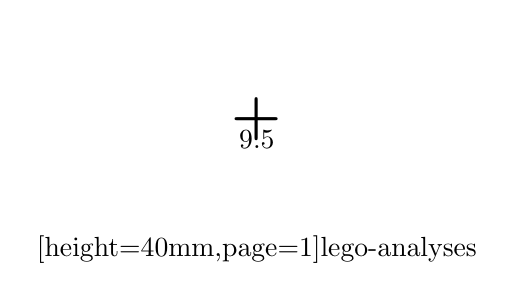
\begin{tikzpicture}
		\node (lego) at (0,-1.7) {\picDark[height=40mm,page=1]{lego-analyses}};
		\node (lego) at (0,-.05) {\huge \textbf{+}};
		\node (lego) at (0,1) {\footnotesize\featureDiagramLego};
		\node at (0,-.3) {\mglass{9.5}};
	\end{tikzpicture}
}

\newcommand{\summaryproductbased}{
	\centering\picDark[width=.8\linewidth,page=9]{lego-analyses}
	\begin{note}{Product-Based Strategy}
		\begin{itemize}
			\item analyze individual \emph{products}
			\item[+] sound, complete
			\item[+] uses off-the-shelf generator\,$\gamma$ and analysis\,$\alpha$
			\item[--] redundant effort
			\item[--] does not scale well
		\end{itemize}
	\end{note}
}

\newcommand{\summaryfeaturebased}{
	\centering\picDark[width=.8\linewidth,page=6]{lego-analyses}
	\begin{note}{Feature-Based Strategy}
		\begin{itemize}
			\item analyze individual \emph{features}
			\item[+] sound, efficient
			\item[--] analysis $\alpha$ requires features with interfaces
			\item[--] incomplete: misses all feature interactions
		\end{itemize}
	\end{note}
}

\newcommand{\summaryfamilybased}{
	\centering\scalebox{.5}{\familybasedlego}
	\begin{note}{Family-Based Strategy}
		\begin{itemize}
			\item analyze the \emph{product line}
			\item[+] sound, complete, efficient
			\item[--] requires careful, hand-crafted analysis $\alpha$
		\end{itemize}
	\end{note}
}

\subsection{Recap: Quality Assurance}

\begin{frame}{\myframetitle\ \mytitlesource{\ludewiglichter}}
	\begin{mycolumns}[widths={45},animation=none]
		\uncover<2->{
			\begin{note}{}
				\begin{itemize}
					\item last lecture:\\
						how to \emph{avoid} variability bugs (esp.~feature interactions)
					\uncover<4->{\item this + next lecture:\\
						how to \emph{find} variability bugs}
				\end{itemize}
			\end{note}
		}
	\mynextcolumn
		\only<1|handout:0>{\picDark[height=\textheightwithtitle,page=1]{quality-assurance}}%
		\only<2|handout:0>{\picDark[height=\textheightwithtitle,page=2]{quality-assurance}}%
		\only<3|handout:0>{\picDark[height=\textheightwithtitle,page=3]{quality-assurance}}%
		\only<4|handout:0>{\picDark[height=\textheightwithtitle,page=4]{quality-assurance}}%
		\only<5|handout:1>{\picDark[height=\textheightwithtitle,page=5]{quality-assurance}}%
		\only<6|handout:0>{\picDark[height=\textheightwithtitle,page=6]{quality-assurance}}%
	\end{mycolumns}
\end{frame}

\widexkcdframe{1700}

\subsection{Automated Analysis of Product Lines}

\begin{frame}{\myframetitle}
	\begin{mycolumns}[t,widths={47}]
		\begin{note}{Typical Program Analyses}
			\begin{mycolumns}[c,animation=none]
				\begin{itemize}
					\item code metrics
					\item type checking
					\item theorem proving
					\item data-flow analysis
					\item performance analysis
					\item \ldots
				\end{itemize}
			\mynextcolumn
				\centering\mglass{3}
			\end{mycolumns}
		\end{note}
		\begin{definition}{What is a Program Analysis?}
			\begin{itemize}
				\item analyzes properties of a \emph{program} (e.g., correctness, performance, and safety)
				\item can be used to automatically find bugs, bottlenecks, and other \emph{vulnerabilities}
			\end{itemize}
		\end{definition}
		\mynextcolumn
		\begin{example}{Asking Questions About Product Lines}
			\begin{itemize}
				\item Which product has the most lines of code? \mysource{\href{https://dl.acm.org/doi/10.1145/3307630.3342384}{ref}}
				\item Which products have type errors? \mysource{\href{https://dl.acm.org/doi/10.1145/1868688.1868693}{ref}}
				\item Which products violate specifications? \mysource{\href{https://dl.acm.org/doi/10.1145/2371401.2371404}{ref}}
				\item Which products have unsafe data flows? \mysource{\href{https://dl.acm.org/doi/10.1145/2499370.2491976}{ref}}
				\item Which is the fastest product? \mysource{\href{https://link.springer.com/article/10.1007/s10515-020-00273-8}{ref}}\\
					Which product has the smallest binary? \mysource{\href{https://dl.acm.org/doi/10.1145/3546932.3546997}{ref}}
				\item \ldots
			\end{itemize}
		\end{example}
		\begin{definition}{What is a Product-Line Analysis?}
			\begin{itemize}
				\item analyzes properties of an entire \emph{product line}
				\item can be roughly classified by its \emph{strategy}:
				\begin{itemize}
					\item product-based
					\item feature-based
					\item family-based
				\end{itemize}
			\end{itemize}
		\end{definition}
	\end{mycolumns}
\end{frame}

\subsection{Product-Based Strategies} % refs missing in whole part!

\begin{frame}{\myframetitle}
	\begin{mycolumns}
		\begin{definition}{Intuition}
			\begin{itemize}
				\item to analyze the product line, just analyze \emph{each product}
				\begin{itemize}
					\item individually
					\item in isolation
					\item possibly in parallel
				\end{itemize}
				\item e.g., compile and verify each product
			\end{itemize}
		\end{definition}
		\begin{exampletight}{}
			\centering\featureDiagramLego\\$Helmet \pimplies \pnot Phone$
		\end{exampletight}
	\mynextcolumn
		\picDark[width=\linewidth,page=9]{lego-analyses}
	\end{mycolumns}
\end{frame}

\begin{frame}{\myframetitle}
	\begin{mycolumns}
		\begin{definition}{Algorithm}
			\begin{algorithmic}
				\Require a product line $pl$; algorithms $\gamma$, $\alpha$, $\sigma$
				\State $C \gets AllSAT(\phi(FM_{pl}))$ \Comment{{\small enumerate valid config's}}
				\State $results \gets []$
				\ForAll{$S \in C$} \Comment{{\small for each valid config}}
				\State $p \gets \gamma(S)$ \Comment{{\small generate product}}
				\State $results \pluseq \alpha(p)$ \Comment{{\small add analysis result}}
				\EndFor
				\State \Return $\sigma(results)$
			\end{algorithmic}
		\end{definition}
		\begin{note}{}
			\begin{itemize}
				\item $\gamma$ \emph{generates} (e.g., compiles) products (e.g., \texttt{make}, \texttt{gradle}, \texttt{FeatureHouse}, \texttt{npm}, \ldots)
				\item $\alpha$ \emph{analyzes} the product (e.g., run verifier)
				\item $\sigma$ \emph{summarizes} the results (e.g., each individual call to $\alpha$ must succeed)
			\end{itemize}
		\end{note}
	\mynextcolumn
		\begin{exampletight}{}
			\begin{center}
				\small\featureDiagramConfigurableDatabase
			\end{center}
		\end{exampletight}
		\begin{example}{}
			\footnotesize
			\begin{mycolumns}[animation=none]
				$\sigma([\alpha(\gamma(\{C,G,W\}))$\\
				$~~~~\alpha(\gamma(\{C,P,W\}))$\\
				$~~~~\alpha(\gamma(\{C,G,P,W\}))$\\
				$~~~~\alpha(\gamma(\{C,D,W\}))$\\
				$~~~~\alpha(\gamma(\{C,G,D,W\}))$\\
				$~~~~\alpha(\gamma(\{C,P,D,W\}))$\\
				$~~~~\alpha(\gamma(\{C,G,P,D,W\}))$\\
				$~~~~\alpha(\gamma(\{C,P,T,W\}))$\\
				$~~~~\alpha(\gamma(\{C,G,P,T,W\}))$\\
				$~~~~\alpha(\gamma(\{C,D,T,W\}))$\\
				$~~~~\alpha(\gamma(\{C,G,D,T,W\}))$\\
				$~~~~\alpha(\gamma(\{C,P,D,T,W\}))$\\
				$~~~~\alpha(\gamma(\{C,G,P,D,T,W\}))$
			\mynextcolumn
				$\alpha(\gamma(\{C,G,L\}))$\\
				$\alpha(\gamma(\{C,P,L\}))$\\
				$\alpha(\gamma(\{C,G,P,L\}))$\\
				$\alpha(\gamma(\{C,D,L\}))$\\
				$\alpha(\gamma(\{C,G,D,L\}))$\\
				$\alpha(\gamma(\{C,P,D,L\}))$\\
				$\alpha(\gamma(\{C,G,P,D,L\}))$\\
				$\alpha(\gamma(\{C,P,T,L\}))$\\
				$\alpha(\gamma(\{C,G,P,T,L\}))$\\
				$\alpha(\gamma(\{C,D,T,L\}))$\\
				$\alpha(\gamma(\{C,G,D,T,L\}))$\\
				$\alpha(\gamma(\{C,P,D,T,L\}))$\\
				$\alpha(\gamma(\{C,G,P,D,T,L\}))])$
			\end{mycolumns}
		\end{example}
	\end{mycolumns}
\end{frame}

\begin{frame}{Classification of Strategies}
	\begin{mycolumns}[t,columns=3,animation=none]
		\summaryproductbased
	\mynextcolumn
	\mynextcolumn
	\end{mycolumns}
\end{frame}

\subsection{Feature-Based Strategies}

% in https://corecursive.com/015-dependant-types-in-haskell-with-stephanie-weirich/#interacting-ghc-extensions, Stephanie Weirich explains how type extensions to the Haskell compiler are often proved correct in isolation, which misses their interactions -> this is basically an example for a feature-based analysis strategy in compiler design

\begin{frame}{\myframetitle}
	\begin{mycolumns}
		\begin{definition}{Intuition}
			\begin{itemize}
				\item to analyze the product line, just analyze \emph{each feature} individually
				\item ignore all relations to other features
				\item e.g., compile and verify each component\\
				$\Rightarrow$ requires \emph{interfaces between features} (components, services, plug-ins) % todo: rename lecture 6 accordingly?
			\end{itemize}
		\end{definition}
		\begin{exampletight}{}
			\centering\featureDiagramLego\\$Helmet \pimplies \pnot Phone$
		\end{exampletight}
	\mynextcolumn
		\picDark[width=\linewidth,page=6]{lego-analyses}
	\end{mycolumns}
\end{frame}

\begin{frame}{\myframetitle}
	\begin{mycolumns}
		\begin{definition}{Algorithm}
			\begin{algorithmic}
				\Require a product line $pl$; algorithms $\alpha$, $\sigma$
				\State $results \gets []$
				\ForAll{$f \in F_{pl}$} \Comment{{\small for each feature}}
				\State $results \pluseq \alpha(f)$ \Comment{{\small add analysis result}}
				\EndFor
				\State \Return $\sigma(results)$
			\end{algorithmic}
		\end{definition}
		\begin{note}{}
			\begin{itemize}
				\item $\alpha$ \emph{analyzes} the feature (e.g., compiles and verifies the component)
				\item $\sigma$ \emph{summarizes} the results (see product-based)
			\end{itemize}
		\end{note}
	\mynextcolumn
		\begin{exampletight}{}
			\begin{center}
				\small\featureDiagramConfigurableDatabase
			\end{center}
		\end{exampletight}
		\begin{example}{}
			\vspace*{-4ex}
			\small
			\begin{align*}
				\sigma([&\alpha(C) \text{ -- e.g., compile and verify base code}\\
				&\alpha(G) \text{ -- e.g., compile and verify feature Get}\\
				&\alpha(P) \text{ -- \ldots}\\
				&\alpha(D)\\
				&\alpha(T)\\
				&\alpha(W)\\
				&\alpha(L)])
			\end{align*}
		\end{example}
	\end{mycolumns}
\end{frame}

\begin{frame}{Classification of Strategies}
	\begin{mycolumns}[t,columns=3,animation=none]
		\summaryproductbased
	\mynextcolumn
		\summaryfeaturebased
	\mynextcolumn
	\end{mycolumns}
\end{frame}

\subsection{Family-Based Strategies}

\begin{frame}{\myframetitle}
	\begin{mycolumns}
		\begin{definition}{Intuition}
			\begin{itemize}
				\item analyze the product line (or \emph{family}) as a whole
				\item requirement: the analysis should give the same result as a product-based analysis
				\item makes use of the feature model and artifacts
				\item analysis is \emph{hand-crafted}, no generic algorithm\\
				$\Rightarrow$ typically: reduction to SAT problems
			\end{itemize}
		\end{definition}
		\begin{example}{Today's Examples}
			\begin{itemize}
				\item analyzing \emph{feature mappings}
				\item analyzing \emph{variable code}
			\end{itemize}
			$\Rightarrow$ here: for \emph{conditional compilation} and \emph{feature-oriented programming}
		\end{example}
	\mynextcolumn
		\centering\familybasedlego
	\end{mycolumns}
\end{frame}

\subsection{Classification of Strategies}

\begin{frame}[label=AnalysisStrategies]{\myframetitle}
	\begin{mycolumns}[t,columns=3,animation=none]
		\summaryproductbased
	\mynextcolumn
		\summaryfeaturebased
	\mynextcolumn
		\summaryfamilybased
	\end{mycolumns}
\end{frame}

\lessonslearned{
	\item product-line analyses are needed for quality assurance
	\item \emph{product-based}: simple, but does not scale
	\item \emph{feature-based}: fairly simple, but misses interactions
	\item \emph{family-based}: efficient, but most complex
}{
	\item \fospl, Chapter 10
	\item \analysisstrategies
}{
	Can you imagine other analysis strategies than product-based, feature-based, and family-based?
	How could such strategies look like?
}

\sectionend

\section{Analyzing Feature Mappings}

%ignoriert völlig Source-Code
% nur Mapping

\subsection{Presence Conditions}

\subsection{Dead Code} % family-based static analysis

% dead code paper (tartler beteiligt, erlangen evtl., TDS+:ATC14/EuroSys11) in linux? technik zum code auskommentieren, nicht alles ist ungewollt

\subsection{Superfluous Annotations}

% Mapping + FM

\subsection{Considering the Feature Model}

% + variability smells erwähnen


\lessonslearned{
	\item feature-mapping analyses alleviate the impact of code scattering and tangling
	\item they are usually not necessary when there is good feature traceability
	\item they cannot detect bugs in the actual code
}{
	\item \fospl, Chapter 10
}{
	Above, we assumed that we know all presence conditions already.
	How can we automatically extract presence conditions from code that uses the C preprocessor?
	What problems might occur?
	% - there might be #includes that contain macro definitions
	% - there might be macros to be expanded, which can get complex quickly
	% - it is not always trivial to distinguish feature macros from compiler- or system-specific macros
	% - there is #undef (or re-#define), which opens another can of worms
	% see works on TypeChef (C. Kästner), SuperC (P. Gazillo), FeatureCoPP (K. Ludwig), PCLocator (E. Kuiter)
}

\sectionend

\section{Analyzing Variable Code}

\subsection{Automated Analysis of Variable Code}

\begin{frame}{\myframetitle}
	\begin{mycolumns}[t,widths={46}]
		\myexample{Asking Questions About\\the Feature Mapping \ldots}{
			\begin{itemize}
				\item Are there contradictory or unnecessary preprocessor annotations in the code?
				\item Is the code even included in any product?
				\item If so, in how many products is the code included?
				\item \ldots
			\end{itemize}
		}
		\mynote{}{
			only finds code-agnostic anomalies
		}
		\mynextcolumn
		\myexample{\ldots\ and the Variable Code}{
			\begin{itemize}
				\item Can every product be generated (e.g., compiled)?\\
					$\Rightarrow$ to find all \emph{syntax and type errors}
				\item Do all tests succeed for every product?\\
					$\Rightarrow$ to find some \emph{runtime and logic errors}
				\item Does every product adhere to its specification?\\
					$\Rightarrow$ to \emph{rule out} runtime and logic errors
				\item \ldots
			\end{itemize}
		}
		\mynote{}{
			now: analyze (non-)functional properties of all products
		}
		\myexample{Today's Example}{
			type checking for FOP and conditional compilation
		}
	\end{mycolumns}
\end{frame}

\subsection{Variability-Aware Type Checking}

\subsubsection{Analyzing Feature Modules}

\begin{frame}{\myframetitle}
	\begin{mycolumns}[widths={37,63},animation=none]
		\myexampletight{}{
			\featureDiagram{Store,abstract[Type,abstract,mandatory[SingleStore,concrete,alternative][MultiStore,concrete]][AccessControl,concrete,optional]}
		}
		\myexample{Feature-Model Formula}{
			\small
			$\Phi(FM) = Store \pand Type \pand (SS \por MS) \pand (\pnot SS \por \pnot MS)$
		}
		\myexample{Valid Configurations}{
			\vspace*{-2ex}
			\small
			\leftandright{
				{\color{black}$\{SS\}$}\\
				$\{SS, AC\}$
			}{
				{\color{black}$\{MS\}$}\\
				$\{MS, AC\}$\\
			}
		}
		\uncover<2->{\mynote{}{
			Is there a type error in \emph{any} product?
			\uncover<3->{What about $\{SS, AC\}$?}
		}}
	\mynextcolumn
		\only<-2>{\pic[width=\linewidth]{fop-csur-example-error-blind}}
	\end{mycolumns}
\end{frame}

\begin{frame}{\myframetitle}
	\begin{mycolumns}[widths={37,63},animation=none]
		\mydefinition{Reachability Condition of $id$}{
			guarantees that a given \emph{reference} to $id$ is also \emph{defined} somewhere:\\[1ex]
			$\Phi(FM) \mimplies (PC_{ref}^{id} \pimplies \bigvee_{def} PC_{def}^{id})$\\[1ex]
			or, with a SAT solver:\\
			\small
			$\pnot SAT(\Phi(FM) \pand PC_{ref} \pand \bigwedge_{def} \pnot PC_{def})$
		}
		\mydefinition{Type-Safe Product-Line}{
			in a \emph{type-safe} SPL, all references must always be defined (i.e., \emph{all} reachability conditions must hold)\\
			{\color{gray}\ldots\ and many more conditions \ldots}
		}
		\myexample{}{
			$\Phi(FM) \mimplies (AC \pimplies SS \por MS)$ holds,\\
			$\Phi(FM) \mimplies (AC \pimplies MS)$ does not\\[1ex]
			$\Rightarrow$ $\{SS, AC\}$ has no \texttt{readAll}!
		}
	\mynextcolumn
		\pic[width=\linewidth]{fop-csur-example-error}
	\end{mycolumns}
\end{frame}

\subsubsection{Analyzing Conditional Compilation}

\begin{frame}[fragile]{\myframetitle}
	\begin{mycolumns}[columns=3,widths={37,29,34},animation=none]
		\myexampletight{}{
			\centering
			\featureDiagram{Graph,concrete[Directed,concrete,optional][Undirected,concrete,optional][Hyper,concrete,optional]}
			{\color{blue}$\pnot (Directed \pand Undirected)$}\\
			{\color{green}$Hyper \pimplies Undirected$}\\
			{\color{red}$Directed \por Hyper$}
		}
		\uncover<2->{\mydefinition{Reachability Condition of $id$}{
			$\Phi(FM) \mimplies (PC_{ref}^{id} \pimplies \bigvee_{def} PC_{def}^{id})$
		}}
		\uncover<3->{\mydefinition{Conflict Condition of $id$, def's $d_i$}{
			guarantees that no definition of $id$ \emph{conflicts} with another:\\[1ex]
			$\Phi(FM) \mimplies \bigwedge_{d_1 \neq d_2} \pnot (PC_{d_1}^{id} \pand PC_{d_2}^{id}))$
		}}
	\mynextcolumn
	\uncover<2->{\myexample{Is $e.nodes$ reachable?}{
			\small
			$\Phi(FM) \mimplies (\top \pimplies$\\
			$~~Dir \por (Hy \pand Un) \por (Hy \pand Dir))$\\[1ex]
			holds, because each graph is {\color{red}directed} or an ({\color{green}undirected}) {\color{red}hypergraph}
		}}
		\uncover<3->{\myexample{Does $e.nodes$ conflict?}{
			\small
			$\Phi(FM) \mimplies ($\\
			$~~\pnot (Dir \pand (Hy \pand Un))$\\
			$~\pand \pnot (Dir \pand (Hy \pand Dir))$\\
			$~~\pand \pnot ((Hy \pand Un) \pand (Hy \pand Dir)))$\\[1ex]
			holds, because a graph is {\color{blue}never} {\color{red}directed} and an ({\color{green}undirected}) {\color{red}hypergraph} {\color{blue}at the same time}
		}}
	\mynextcolumn
		\begin{uncoverenv}<2->
			\begin{cpptight}[basicstyle=\small]{\texttt{graph.cpp}}
class Node { ... };

class Edge {
#ifdef DIRECTED
	pair<Node, Node> nodes;
#endif
#ifdef HYPER
#ifdef UNDIRECTED
	set<Node> nodes;
#endif
#ifdef DIRECTED
	map<Node, set<Node>> nodes;
#endif
#endif
};

std::ostream& operator<<(
	std::ostream &s, const Edge &e) {
	return s << e.nodes;
}
			\end{cpptight}
		\end{uncoverenv}
	\end{mycolumns}
\end{frame}

\subsubsection{Discussion}

\begin{frame}{\myframetitle}
	\begin{mycolumns}
		\mynote{Just the Tip of the Iceberg}{
			\begin{itemize}
				\item here, we only discussed reachability and conflict conditions
				\item but: actual type checking requires a table of all identifiers, their types, and their PCs (and a lot more SAT queries)
				\item the practical difficulty depends:
				\begin{itemize}
					\item FOP (due to superimposition)\\
						$\Rightarrow$ no conflict conditions required
					\item good feature traceability (e.g., FOP)\\
						$\Rightarrow$ trivial PCs, simpler implementation
					\item ignoring the feature model\\
						$\Rightarrow$ better performance (false positives!)
				\end{itemize}
			\end{itemize}
		}
	\mynextcolumn
		\myexample{The TypeChef Project \mysource{\typechef}}{
			\begin{itemize}
				\item a variability-aware lexer, parser framework, and type system for C code with \texttt{\#ifdef}'s
				\item skips preprocessing, instead builds an abstract syntax tree (AST) annotated with presence conditions
				\item \href{https://ckaestne.github.io/TypeChef/typechef-poster.png}{poster} with examples
				\item does it scale?\\[1ex]
				{\small Busybox (811 features): \mycite{We need 57 minutes to type check all modules.}} \mysource{\href{https://dl.acm.org/doi/10.1145/2384616.2384673}{ref}}\\[1ex]
				{\small Linux (6065 features): \mycite{We successfully parsed [it in] roughly 85 hours on a single machine.}} \mysource{\href{https://dl.acm.org/doi/10.1145/2048066.2048128}{ref}} % not practically possible, can be used to motivate testing in next lecture
			\end{itemize}
		}
	\end{mycolumns}
\end{frame}

\subsection{Product-Line Analyses in the Wild}

\subsubsection*{Product-Line Complexity}

\begin{frame}{\myframetitle}
	\leftorright{
		\mydefinition{Six Classes of Product-Line Complexity \mytitlesource{\href{https://youtu.be/qUuRp7_d0rU?t=1651}{Thüm~2021}}}{
			In a timeframe of 24h \ldots
			\begin{enumerate}
				\item[\color{gray}\textbf{NC}] {\color{gray}Products cannot be generated automatically}
				\item[\textbf{C1}] All products can be generated and \emph{tested}
				\item[\textbf{C2}] Not C1, but all \emph{products} can be \emph{generated}
				\item[\textbf{C3}] Not C2, but all \emph{configurations} can be \emph{generated} (AllSAT)
				\item[\textbf{C4}] Not C3, but the \emph{number of valid configurations} can be computed (\ssat{})
				\item[\textbf{C5}] Not C4, but \emph{whether there is a valid configuration} can be computed (SAT)
				\item[\textbf{C6}] It cannot be computed whether there is a valid configuration
			\end{enumerate}
		}
	}{
		\myexample{Examples}{
			% also put examples of analysis strategies here, and which kind of mapping/code analysis scales for which class?
			\begin{enumerate}
				\item[\color{gray}\textbf{NC}] {\color{gray}all product lines with custom development in application engineering\\(e.g., components and services with glue code, white-box frameworks)}
				\item[\textbf{C1}] $< 2000$ products for 1 min per product
				\item[\textbf{C2}] $< 90000$ products for 1 s per product
				\item[\textbf{C3}] $< 10^{13}$ configurations for 1 ns per configuration
				\item[\textbf{C4}] older versions of Linux/Automotive05
				\item[\textbf{C5}] newer versions of Linux/Automotive05\\(see \evaluatingsharpsatsolvers)
				\item[\textbf{C6}] No example known
			\end{enumerate}
		}
	}
\end{frame}

\subsubsection*{Automated Analysis \ldots}

\begin{frame}{\myframetitle}
	\begin{mycolumns}[t,columns=3]
		\textbf{Lecture 4.3}
		\mydefinition{\ldots\ of Feature Models}{
			analyze only the feature model
		}
	\mynextcolumn
		\textbf{Lecture 10.2}
		\mydefinition{\ldots\ of Feature Mappings}{
			analyze the feature mapping (considering the feature model)
		}
	\mynextcolumn
		\textbf{Lecture 10.3}
		\mydefinition{\ldots\ of Variable Code}{
			analyze the variable code (considering the feature model and feature mapping)
		}
	\end{mycolumns}
	\begin{mycolumns}[t,columns=3]
		\myexample{}{
			\begin{itemize}
				\item void, core/dead features
				\item decision propagation
				\item atomic sets, redundant constraints
				\item \ldots
			\end{itemize}
		}
	\mynextcolumn
		\myexample{}{
			\begin{itemize}
				\item dead code
				\item superfluous annotations
				\item degree of code scattering and tangling
				\item \ldots
			\end{itemize}
		}
	\mynextcolumn
		\myexample{}{
			\begin{itemize}
				\item parsing, type checking
				\item static analysis
				\item model checking, theorem proving
				\item \ldots
			\end{itemize}
		}
	\end{mycolumns}
	\begin{mycolumns}[t,columns=2,widths={32}]
	\mynextcolumn
		\mynote{}{
			here: \emph{family-based} analysis strategies for \emph{conditional compilation} and \emph{feature-oriented programming}
		}
	\end{mycolumns}
\end{frame}

\lessonslearned{
	\item \todots
}{
	\item \todots
}{
	\todots
}

\mode<beamer>{
	\begin{frame}{\inserttitle}
		\lectureseriesoverview
	\end{frame}

	\contentoverview
}


\end{document}
